\documentclass[conference]{IEEEtran}
\IEEEoverridecommandlockouts
\usepackage{graphicx}
\usepackage{booktabs}
\usepackage{amsmath}
\usepackage{multirow}
\usepackage[hidelinks]{hyperref}
\usepackage{xcolor}

\begin{document}

\title{Detect, Refine, Vote: Robustly Validated Instance Segmentation of Solar Filaments in GONG H$\alpha$ Images}

% TODO(author): fill in affiliation and contact details before submission.
\author{\IEEEauthorblockN{Trishanth Mellimi}
\IEEEauthorblockA{\textit{[Department], [Institution]}\\
[City], [Country] \\
[email]}}

\maketitle

\begin{abstract}
Solar filaments are the cores of many eruptions that drive space weather, yet segmenting them as individual instances in full-disk H$\alpha$ images remains hard: they are thin, faint at their ends, and annotators disagree about which ones to mark. We describe our solution to the IEEE BigData Cup 2026 Solar Filament Segmentation Challenge (MAGFiLO, panoptic quality). It is a detect--refine--vote pipeline: four instance detectors propose filaments, an ImageNet-pretrained crop refiner supervised with the dataset's filament spines draws each mask, per-source isotonic calibration and cross-source non-maximum suppression select detections, and a cluster-level weighted pixel vote over overlapping masks from all sources (including a native-resolution semantic U-Net whose spine-seeded instances act as extra detections) produces the final segmentation. Every design choice was accepted only if it improved out-of-fold panoptic quality on five random calibration splits with a paired bootstrap. The pipeline reaches PQ 0.40 on the public leaderboard without using any test annotations; the voting stage with semantic leaders adds +0.0115 PQ over the calibrated detector ensemble on held-out data, positive on all five splits. We also measure that two human annotators of the same image agree at only PQ 0.34, while our model scores 0.46 against a held-out annotator, which bounds the headroom left in this benchmark.
\end{abstract}

\begin{IEEEkeywords}
solar filaments, instance segmentation, panoptic quality, ensemble, H-alpha, space weather
\end{IEEEkeywords}

\section{Introduction}
Filaments are dense, cool plasma suspended by magnetic fields above polarity inversion lines; they appear as dark, elongated features on the H$\alpha$ disk and are at the core of coronal mass ejections and solar flares. Automated, instance-level segmentation of filaments in the continuous full-disk H$\alpha$ stream of the Global Oscillation Network Group (GONG)~\cite{harvey1996gong} is therefore of direct interest to space-weather forecasting. The MAGFiLO dataset~\cite{ahmadzadeh2024magfilo} provides manually annotated filament polygons and spines for GONG images, and the IEEE BigData Cup 2026 challenge built on it asks for instance segmentations scored by panoptic quality (PQ)~\cite{kirillov2019panoptic}.

Three properties make the task harder than generic instance segmentation: filaments are thin (often a few pixels wide in a $2048\times2048$ image) and fade gradually at their ends; neighbouring filaments touch or fragment; and the labels are noisy, since 42\% of training images were annotated by two or three people who often disagree on which structures are filaments. Prior deep-learning filament detectors combine object detection with semantic segmentation~\cite{diercke2024universal}; we follow the same two-stage idea but build it as a calibrated ensemble.

Our contributions are: (i) a detect--refine--vote pipeline whose final stage replaces ``keep the best-scoring mask'' with a score-weighted pixel vote over all overlapping candidates, with detection (leader) and voting roles assigned separately; (ii) an evaluation protocol based on out-of-fold calibration and paired bootstrap over five random splits, which rejected most of the roughly 50 variants we tried, including several that looked better on a single split; and (iii) a quantitative account of where the remaining error lies, including the human inter-annotator agreement on the same metric.

\section{Data and Evaluation Protocol}
\textbf{Data.} The challenge training set contains 707 GONG H$\alpha$ images ($2048\times2048$, six observatories, 2011--2022) with 1,154 annotation sets (an image annotated by $k$ people appears $k$ times) and 8,199 filament polygons, each with a spine polyline. The test set has 180 images; the public leaderboard is computed on about half of them. We used only the challenge-provided annotations; no MAGFiLO test annotations were used at any point.

\textbf{Split.} We hold out 10\% of the \emph{images} (70 images, 116 annotation sets, 908 filaments) for validation, so that no image appears on both sides through a second annotator. Each annotation set is scored separately, which matches the challenge's per-image ground truth.

\textbf{Metric.} PQ $=\sum_{(y,\hat y)\in TP}\mathrm{IoU}(y,\hat y)\,/\,(|TP|+\frac12|FP|+\frac12|FN|)$ with matches at IoU $>0.5$, pooled over all images, implemented as in the organizers' self-evaluation notebook. We also report its factors, segmentation quality (SQ, mean IoU of matches) and recognition quality (RQ).

\textbf{Robustness protocol.} The pipeline has calibration models and thresholds fitted on validation data, so in-sample scores are optimistic. For every comparison we (a) split the validation images into two folds, fit calibrators on one and score the other, (b) repeat for five random fold assignments, and (c) compute a 2,000-sample paired bootstrap of the per-image PQ difference. With 116 annotation sets the 95\% interval of a PQ difference is roughly $\pm0.01$; we kept a change only if it was positive on all five splits.

\section{Method}
Fig.~\ref{fig:pipeline} summarizes the pipeline.

\begin{figure*}[t]
\centering
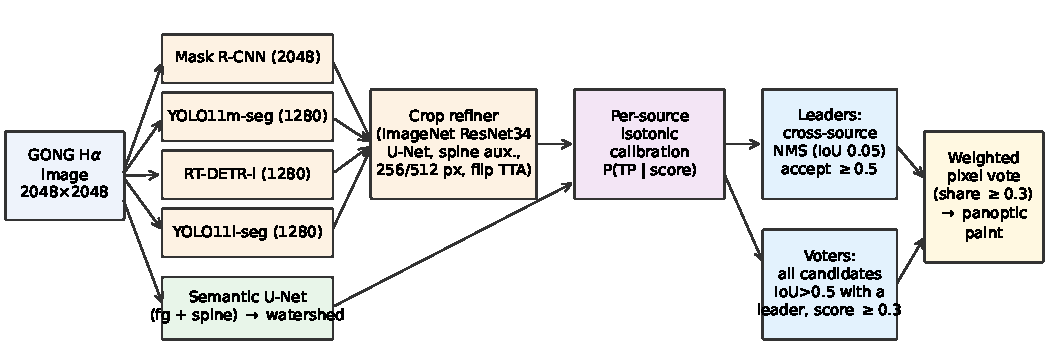
\includegraphics[width=\textwidth]{fig_pipeline.pdf}
\caption{Detect--refine--vote pipeline. Detector proposals are re-segmented by a crop refiner, scores are calibrated per source, cross-source NMS selects leaders, and each leader's final mask is a score-weighted pixel vote over all overlapping candidates. The semantic U-Net's instances act as additional leaders and voters.}
\label{fig:pipeline}
\end{figure*}

\subsection{Instance detectors}
We train four detectors with different architectures and input scales: Mask R-CNN~\cite{he2017maskrcnn} (torchvision ResNet-50-FPN v2, COCO-initialized) at the native $2048$\,px resolution; YOLO11m-seg and YOLO11l-seg~\cite{jocher2024yolo11} at 1280\,px; and RT-DETR-l~\cite{zhao2024rtdetr} at 1280\,px. A recurring failure was that well-localized boxes received very low confidence, so we up-weighted the classification loss (3$\times$ for Mask R-CNN, \texttt{cls}$=1.5$ for YOLO, \texttt{cls}$=2.0$ for RT-DETR); for RT-DETR this raised the median score of well-localized boxes from 0.03 to 0.66. Running Mask R-CNN at native resolution instead of downscaling to 1333\,px improved the ensemble by +0.0035 PQ on all five splits.

\subsection{Crop refiner}
Detector mask heads are coarse, so every proposal is re-segmented by a refiner: a square crop of $1.8\times$ the proposal's extent is resized to $256\times256$ (a second refiner uses $512\times512$) and passed to a U-Net~\cite{ronneberger2015unet} with an ImageNet-pretrained ResNet-34 encoder~\cite{he2016resnet,iakubovskii2019smp}. Besides the mask, the refiner predicts the annotated spine (centerline) as an auxiliary output, which steers features toward the filament's axis. It is trained on crops around ground-truth instances with BCE+Dice (weight 0.7) and spine BCE (0.3), and applied with four-view flip test-time augmentation. Replacing an equally-sized from-scratch U-Net by the pretrained encoder reduced validation loss from 0.103 to 0.092 and improved the full ensemble by +0.006 to +0.012 PQ on all five splits (mean +0.009), the largest gain of any single component.

\subsection{Semantic model}
Following a suggestion from the challenge forum that a well-trained segmentation network is competitive, we train a U-Net with an ImageNet ConvNeXt-Tiny encoder~\cite{liu2022convnext} at \emph{native} resolution on $1024\times1024$ crops, with focal~\cite{lin2017focal} plus Dice~\cite{milletari2016vnet} loss on the foreground and BCE plus Dice on a 5\,px rasterized spine, dihedral and on-disk photometric augmentation, AdamW and a cosine schedule (62 epochs, 3\,h on one GPU). Instances are obtained by thresholding the foreground at 0.5, using connected components of the spine map ($>0.3$) as watershed seeds to split touching filaments, and dropping regions under 100\,px; an instance's score is its mean foreground probability.

\subsection{Calibration, selection and cluster voting}
Raw scores are not comparable across detectors, so each source's scores are mapped to $P(\mathrm{TP}\mid\text{score})$ by isotonic regression~\cite{zadrozny2002calibration} fitted on validation candidates (a candidate is a TP if its refined mask has IoU $>0.5$ with an annotated filament). Candidates from all leader sources are pooled, and a greedy NMS keeps those with calibrated score $\ge0.5$ that overlap no previously kept candidate by more than IoU 0.05; we call the survivors \emph{leaders}.

Rather than keeping only each leader's own mask, we fuse it with the masks that describe the same filament, in the spirit of weighted box fusion~\cite{solovyev2021wbf}. Every non-leader candidate with calibrated score $\ge0.3$ joins the leader it overlaps most if that IoU exceeds 0.5. The leader's final mask contains the pixels whose score-weighted share of the cluster's masks is at least 0.3. Detection and voting roles are assigned separately. The leaders are the four detectors (refined at 256\,px) plus the semantic instances. The voters are the leaders plus the same four detectors refined at 512\,px and run on the horizontally mirrored image. Finally, masks are painted in score order onto an instance map so that predictions do not overlap (fragments under 20\,px are dropped).

\section{Experiments}

\begin{table}[t]
\centering
\caption{Validation results (calibration fitted on the full validation split). $\Delta$ OOF: out-of-fold PQ change versus the 4-detector baseline, range over five random calibration splits (all positive).}
\label{tab:main}
\setlength{\tabcolsep}{3.2pt}
\begin{tabular}{lcccc}
\toprule
Configuration & PQ & SQ & RQ & $\Delta$ OOF \\
\midrule
Mask R-CNN (2048 px) & .432 & .682 & .633 & \\
YOLO11m-seg & .437 & .685 & .638 & \\
RT-DETR-l & .439 & .686 & .639 & \\
YOLO11l-seg & .427 & .686 & .621 & \\
Semantic U-Net (instances) & .406 & .667 & .608 & \\
\midrule
4 detectors, calibrated NMS & .456 & .682 & .668 & --- \\
+ cluster vote, 4 voters & .460 & .682 & .675 & +.003\,/\,+.004 \\
+ cluster vote, 12 voters & .462 & .684 & .676 & +.005\,/\,+.009 \\
+ semantic leader, 5 voters & .461 & .680 & .678 & +.001\,/\,+.009 \\
+ semantic leader, 13 voters & \textbf{.468} & .683 & \textbf{.685} & +.007\,/\,+.016 \\
\bottomrule
\end{tabular}
\end{table}

\textbf{Main results.} Table~\ref{tab:main} lists single sources and the stages of the pipeline. Each detector alone reaches PQ 0.43--0.44; the calibrated ensemble of four reaches 0.456, mainly through recognition (RQ 0.668 vs.\ $\le$0.639). Cluster voting improves SQ and converts near misses into matches, and the semantic instances, which find filaments the detectors miss, add recall once their rough shapes are cleaned up by the vote (matched filaments rise from 570 to 603 of 908). The full configuration improves on the 4-detector baseline by +0.007 to +0.016 PQ out of fold (mean +0.0115). On the public leaderboard the 4-detector baseline and all voting variants score 0.40; with $\sim$90 public images and two-decimal reporting, differences of this size are not resolvable there, and our validation scores run about 0.05 above the public ones for every configuration.

\textbf{What did not help.} Table~\ref{tab:neg} lists the main rejected alternatives. Two patterns recur. First, adding \emph{detections} from additional correlated sources (a second-seed Mask R-CNN, mirrored-image proposals, the semantic instances without voting) adds near-duplicate false positives faster than true positives; the same sources help when they only vote. Second, learned rescoring with richer features improves candidate-level ranking but not PQ, and lowering the acceptance threshold does not pay off.

\begin{table}[t]
\centering
\caption{Rejected alternatives (validation PQ; OOF ranges over five splits where available).}
\label{tab:neg}
\setlength{\tabcolsep}{3pt}
\begin{tabular}{p{4.9cm}p{2.9cm}}
\toprule
Alternative & Effect \\
\midrule
Mask2Former (Swin-T), frozen or unfrozen encoder & solo $\le$.345; lowers ensemble \\
SAM ViT-B, box-prompted decoder fine-tune & .316 \\
SimSiam pretraining on 4k unlabeled GONG images & tie; public .38 \\
Self-training on pseudo-labeled test images & .417 $\rightarrow$ .393 \\
CLAHE contrast enhancement & .425 $\rightarrow$ .412--.419 \\
Gradient-boosted rescorer (agreement, shape) & $-$.014 to $-$.004 \\
Mask growing into U-Net foreground & helps weak refiner, $-$.006 with pretrained one \\
Mirrored-image proposals as detections & $-$.009 to $+$.003 \\
Second-seed or augmented Mask R-CNN & $-$.005 to $+$.003 \\
Two semantic models averaged & $-$.006 to $-$.003 \\
\bottomrule
\end{tabular}
\end{table}

\textbf{Where the error is.} For the 4-detector baseline, 325 of 908 validation filaments are missed. For 219 of them a correct mask exists in the candidate pool but its calibrated score is below the acceptance threshold (median 0.33); 67 have no correct candidate (57 of these have a near miss at IoU 0.3--0.5, typically a mask truncated before the filament's faint tail); 39 were suppressed by an overlapping wrong candidate. Lowering the threshold does not help: leaders scored 0.3--0.5 are true positives at most 32\% of the time even when nine or more sources agree, below the $\approx$0.34 rate at which accepting a detection increases PQ.

\textbf{Human agreement.} On the 296 training images annotated by two or more people, scoring one annotator against another with the challenge metric gives PQ 0.340 (SQ 0.634, RQ 0.536), and 0.309 on the 33 validation images with multiple annotators. Our model scores 0.456--0.468 against a held-out annotator, i.e., it agrees with a single annotator better than annotators agree with each other: trained on all annotators, it learns their consensus. Much of the remaining ``error'' is therefore disagreement about which faint structures are filaments and where their tails end, which bounds what any method can gain on this metric.

\begin{figure*}[t]
\centering
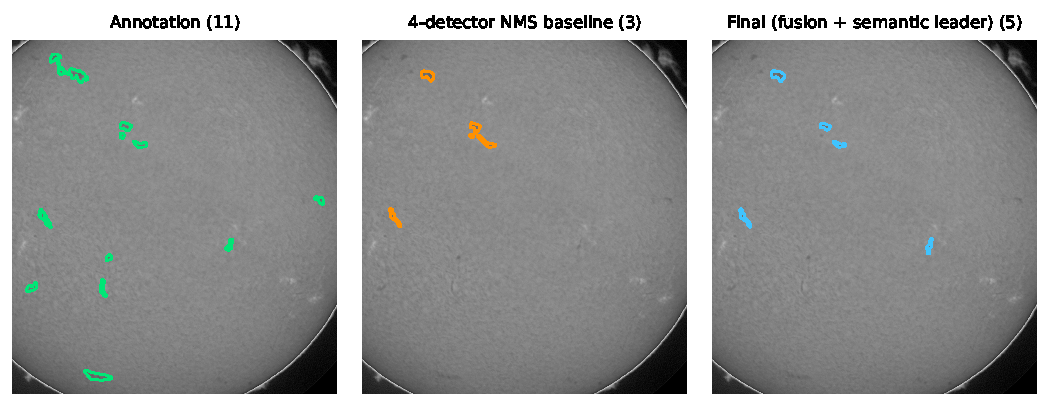
\includegraphics[width=\textwidth]{fig_qualitative.pdf}
\caption{Validation example where voting helps (chosen as the image with the largest gain in matched filaments). Left: one annotator's filaments. Middle: the 4-detector baseline merges two filaments into one instance and misses several faint ones. Right: the final pipeline separates the pair and recovers two more; several faint annotated filaments remain undetected.}
\label{fig:qual}
\end{figure*}

\section{Discussion}
\textbf{Validation discipline.} Most variants we tried looked better on one split and failed out of fold, and several one-split ``wins'' also failed on the leaderboard. Requiring a positive change on every random calibration split, rather than optimizing a single score, was what separated real gains (pretrained refiner, cluster voting, semantic leaders) from noise.

\textbf{Cost.} The full configuration runs each detector twice (original and mirrored image), the crop refiner three times per proposal, and the semantic U-Net once. A light configuration that keeps the semantic leader but only the five leader sources as voters retains about 40\% of the gain (+0.005 PQ out of fold) at substantially lower inference cost.

\textbf{Limitations.} Fine-scale barbs are still largely missed: the refiner works at 256--512\,px per crop and the semantic model at native resolution, but neither is trained to emphasize barbs, which are thin and inconsistently annotated. The 0.05 gap between validation and public scores is consistent across configurations and is also reported by other participants; we have not identified its cause.

\section{Conclusion}
A carefully calibrated ensemble of standard detectors, a pretrained spine-supervised crop refiner, and a cluster-level pixel vote that separates detection from voting roles yields robust, if incremental, gains in PQ for solar filament segmentation, reaching 0.40 on the public leaderboard without test-label leakage. The measured human inter-annotator agreement (PQ 0.34) suggests that progress on this benchmark should be judged with out-of-fold protocols and distributional measures rather than leaderboard differences of a few thousandths.

% TODO(author): IEEE requires disclosing AI-generated content; adjust to describe how AI tools were actually used.
\section*{Acknowledgment}
We thank the organizers of the IEEE BigData Cup 2026 Solar Filament Segmentation Challenge and the MAGFiLO team for the data. AI-based coding assistants were used for implementing and running experiments and for drafting text; all design decisions, results, and claims were reviewed by the author.

\bibliographystyle{IEEEtran}
\begin{thebibliography}{99}
\bibitem{harvey1996gong} J.~W. Harvey \emph{et al.}, ``The Global Oscillation Network Group (GONG) project,'' \emph{Science}, vol.~272, no.~5266, pp.~1284--1286, 1996.
\bibitem{ahmadzadeh2024magfilo} A.~Ahmadzadeh \emph{et al.}, ``A dataset of manually annotated filaments from H-alpha observations,'' \emph{Scientific Data}, vol.~11, art.~1031, 2024, doi: 10.1038/s41597-024-03876-y.
\bibitem{kirillov2019panoptic} A.~Kirillov, K.~He, R.~Girshick, C.~Rother, and P.~Doll\'ar, ``Panoptic segmentation,'' in \emph{Proc. CVPR}, 2019, pp.~9404--9413.
\bibitem{diercke2024universal} A.~Diercke \emph{et al.}, ``A universal method for solar filament detection from H$\alpha$ observations using semi-supervised deep learning,'' \emph{Astron. Astrophys.}, vol.~686, art.~A213, 2024, doi: 10.1051/0004-6361/202348314.
\bibitem{he2017maskrcnn} K.~He, G.~Gkioxari, P.~Doll\'ar, and R.~Girshick, ``Mask R-CNN,'' in \emph{Proc. ICCV}, 2017, pp.~2961--2969.
\bibitem{jocher2024yolo11} G.~Jocher and J.~Qiu, ``Ultralytics YOLO11,'' 2024. [Online]. Available: https://github.com/ultralytics/ultralytics
\bibitem{zhao2024rtdetr} Y.~Zhao \emph{et al.}, ``DETRs beat YOLOs on real-time object detection,'' in \emph{Proc. CVPR}, 2024, pp.~16965--16974.
\bibitem{ronneberger2015unet} O.~Ronneberger, P.~Fischer, and T.~Brox, ``U-Net: Convolutional networks for biomedical image segmentation,'' in \emph{Proc. MICCAI}, 2015, pp.~234--241.
\bibitem{he2016resnet} K.~He, X.~Zhang, S.~Ren, and J.~Sun, ``Deep residual learning for image recognition,'' in \emph{Proc. CVPR}, 2016, pp.~770--778.
\bibitem{iakubovskii2019smp} P.~Iakubovskii, ``Segmentation Models Pytorch,'' 2019. [Online]. Available: https://github.com/qubvel/segmentation\_models.pytorch
\bibitem{liu2022convnext} Z.~Liu, H.~Mao, C.-Y. Wu, C.~Feichtenhofer, T.~Darrell, and S.~Xie, ``A ConvNet for the 2020s,'' in \emph{Proc. CVPR}, 2022, pp.~11976--11986.
\bibitem{lin2017focal} T.-Y. Lin, P.~Goyal, R.~Girshick, K.~He, and P.~Doll\'ar, ``Focal loss for dense object detection,'' in \emph{Proc. ICCV}, 2017, pp.~2980--2988.
\bibitem{milletari2016vnet} F.~Milletari, N.~Navab, and S.-A. Ahmadi, ``V-Net: Fully convolutional neural networks for volumetric medical image segmentation,'' in \emph{Proc. 3DV}, 2016, pp.~565--571.
\bibitem{zadrozny2002calibration} B.~Zadrozny and C.~Elkan, ``Transforming classifier scores into accurate multiclass probability estimates,'' in \emph{Proc. KDD}, 2002, pp.~694--699.
\bibitem{solovyev2021wbf} R.~Solovyev, W.~Wang, and T.~Gabruseva, ``Weighted boxes fusion: Ensembling boxes from different object detection models,'' \emph{Image Vis. Comput.}, vol.~107, art.~104117, 2021.
\end{thebibliography}

\end{document}
